%!TEX root = ../../thesis.tex
\chapter{Implementation}

\section{Brain Tumor detection model}
 
\subsection{Introduction}
 
 In this model, We utilize two primary datasets, Br35H \cite{br35h} and a dataset from Huggingface [3], which contain a variety of brain MRI images categorized into negative (no tumor) and positive (tumor) samples. The following sections provide a detailed explanation of the dataset selection, preprocessing, and configuration.
 
\subsubsection{Datasets details}

The datasets available for this project are: 

\begin{enumerate}
    \item Br35h \cite{br35h}: This dataset consists of 1500 negative and 1500 positive samples.
    \item Huggingface: This dataset comprises 1312 negative and 4057 positive samples.
\end{enumerate}


\subsection{Dataset Configuration Parameters}

The training script allows the customization of various dataset parameters through configurable options. These parameters include the choice of the dataset, the limit on the number of samples, the option to split large datasets, the percentage of data used for testing, and whether to clean previous runs and augment samples \ref{fig:brain_tumor_data_conf}.

\begin{figure}
    \centering
    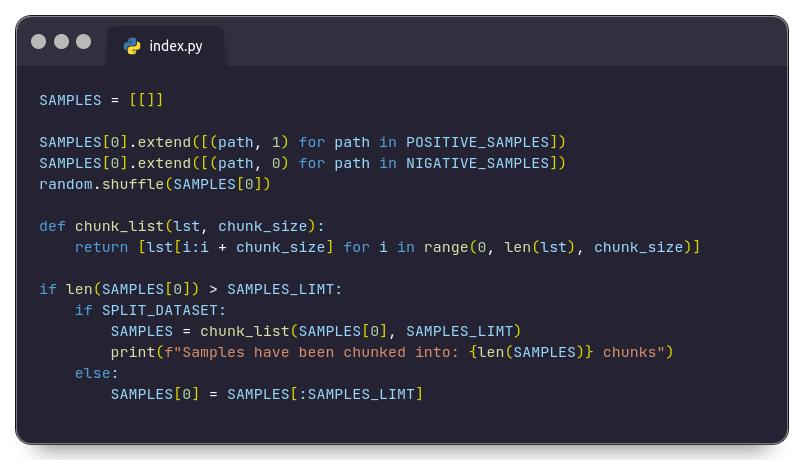
\includegraphics[width=0.90\textwidth]{Img/Chap-01/18.jpg}
    \caption{Dataset configuration}
    \label{fig:brain_tumor_data_conf}
\end{figure}

\subsection{Dataset Preparation}

The dataset preparation process includes downloading the chosen dataset, copying samples, and organizing them into positive and negative categories. Based on the dataset selected (Br35H or Huggingface), appropriate functions are called to fetch and prepare the data.

\subsubsection{Data Shuffling and Splitting}

The samples are shuffled, and if the total number of samples exceeds the limit, they are either split into chunks or truncated based on the configuration, to improve the learning performance \ref{fig:brain_tumor_data_suffiling}.

\begin{figure}
    \centering
    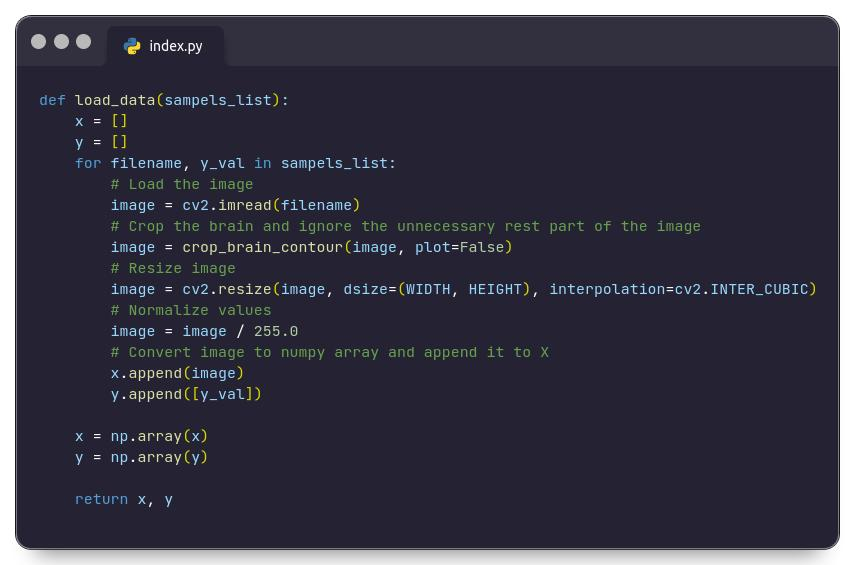
\includegraphics[width=0.90\textwidth]{Img/Chap-01/19.jpg}
    \caption{ Data shuffling}
    \label{fig:brain_tumor_data_suffiling}
\end{figure}

This concludes the dataset settings and preparation chapter. The next steps involve utilizing these prepared datasets to train and evaluate our AI model for brain tumor detection. 

\subsubsection{Edges Cropping}

To enhance the accuracy of brain tumor detection, it is essential to focus on the region of interest (ROI), which in this case is the brain itself. We implemented a cropping technique to isolate the brain from the rest of the image by finding the extreme points of the brain contour. This section details the cropping method, which is based on the approach described in [Finding extreme points in contours with OpenCV.

\subsubsection{Cropping Methodology}

\begin{enumerate}[i)]
    \item Convert to Grayscale and Blur: 
        \begin{itemize}
            \item The input image is converted to grayscale to simplify the processing.
            \item A Gaussian blur is applied to the grayscale image to reduce noise and detail, which helps in thresholding.
        \end{itemize}
    \item Thresholding: 
        \begin{itemize}
            \item A binary threshold is applied to the blurred image, converting it into a binary image where the brain region becomes white (255) and the background becomes black (0). 
            \item Erosion and dilation operations are performed to remove small noise and smooth the object boundaries. 
        \end{itemize}
    \item Finding Contours: Contours are identified in the binary image, and the largest contour is assumed to be the brain region. 
    \item Extreme Points Calculation: The extreme left, right, top, and bottom points of the brain contour are identified.
    \item Cropping the Image: Using the extreme points, the original image is cropped to extract the brain region.
\end{enumerate}


\subsection{Load and Resizing}

To feed the images into our AI model, it is crucial to prepare and resize them to a consistent shape. The `load\_data` function takes a list of image file paths and labels, preprocesses the images, and returns the data in a format suitable for training \ref{fig:brain_tumor_loaddata}

 \begin{figure}
    \centering
    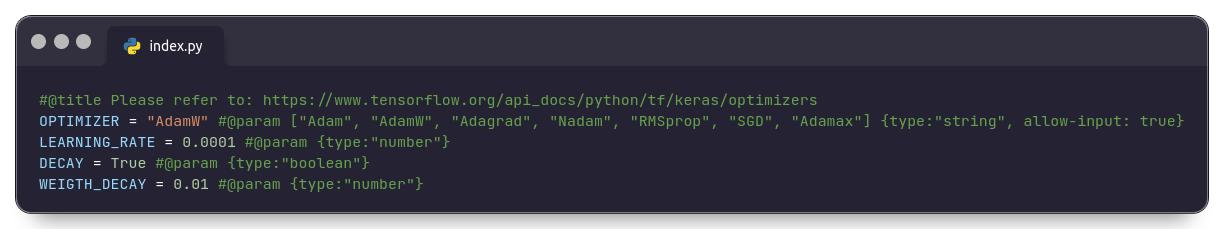
\includegraphics[width=0.90\textwidth]{Img/Chap-01/20.jpg}
    \caption{ The load data function}
    \label{fig:brain_tumor_loaddata}
\end{figure}

\subsubsection{Explanation}

\begin{enumerate}
    \item Loading the Image: Each image is loaded using `cv2.imread`.
    \item Cropping the Brain Region: The function `crop brain contour` is called to crop the brain region from the image. 
    \item Resizing the Image: The cropped image is resized to the specified `WIDTH` and `HEIGHT` using cubic interpolation. 
    \item Normalization: The pixel values of the image are normalized to the range [0, 1] by dividing by 255.0.
    \item Appending to Lists: The processed image and its corresponding label are appended to lists `x` and `y`, respectively. 
    \item Conversion to Numpy Arrays: The lists `x` and `y` are converted to NumPy arrays for efficient processing and handling in machine learning models.
\end{enumerate}

\section{Model Building}

\subsection{Model parameters}

We can select the optimizer and set its parameters through the \ref{fig:brain_tumor_model_params} code snippet.

\begin{figure}
    \centering
    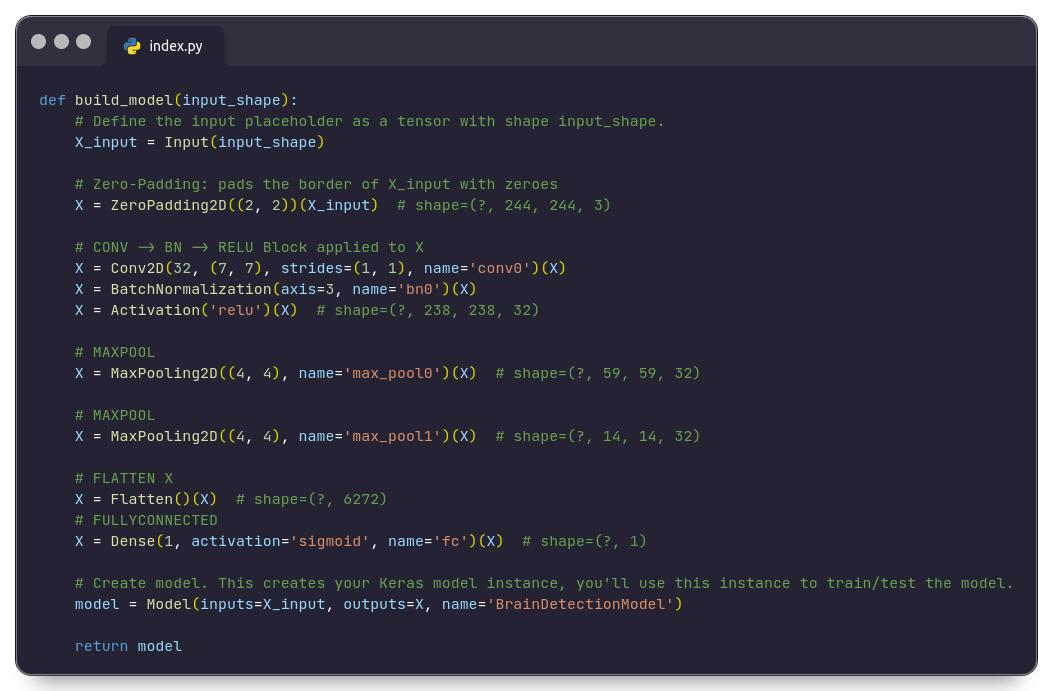
\includegraphics[width=0.90\textwidth]{Img/Chap-01/21.jpg}
    \caption{ The CNN model parameters}
    \label{fig:brain_tumor_model_params}
\end{figure}

\subsection{The building function}

The `build model` function defines the architecture of the CNN, code snippet \ref{fig:brain_tumor_model_architecture}. 

\begin{figure}
    \centering
    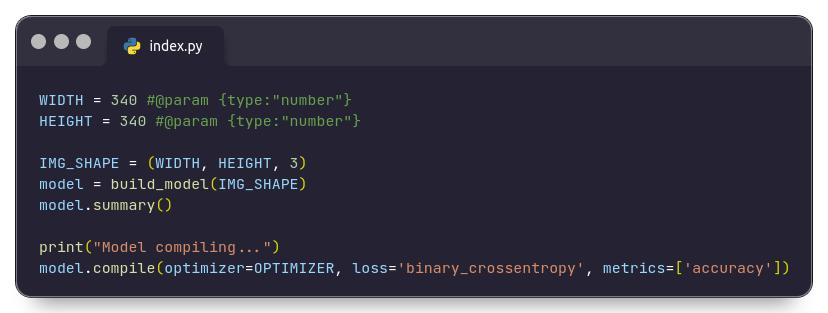
\includegraphics[width=0.90\textwidth]{Img/Chap-01/22.jpg}
    \caption{ The model architecture}
    \label{fig:brain_tumor_model_architecture}
\end{figure}

\subsection{Model Compilation}

After building the model, it needs to be compiled with the chosen optimizer, loss function, and metrics, code snippet \ref{fig:brain_tumor_compilation}.

\begin{figure}
    \centering
    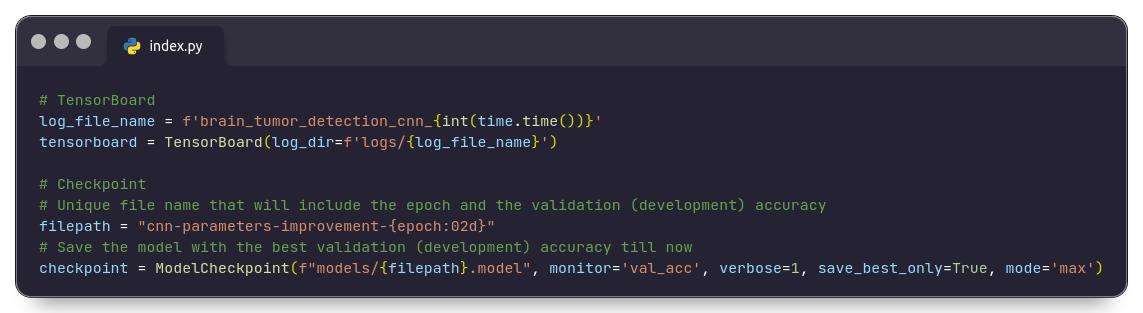
\includegraphics[width=0.90\textwidth]{Img/Chap-01/23.jpg}
    \caption{CNN model compilation}
    \label{fig:brain_tumor_compilation}
\end{figure}

\subsection{ Callbacks}
To monitor the training process and save the best model, we use TensorBoard and ModelCheckpoint callbacks, code snippet \ref{fig:brain_tumor_callbacks}

\begin{figure}
 \centering
    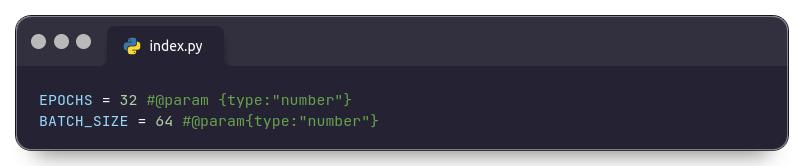
\includegraphics[width=0.90\textwidth]{Img/Chap-01/24.jpg}
    \caption{Setup the callbacks}
    \label{fig:brain_tumor_callbacks}
\end{figure}

\subsection{Summary}
This section covers the crucial steps of building and compiling the CNN model for brain tumor detection. By allowing us to select the optimizer and its parameters, we ensure flexibility in training. Additionally, callbacks are set up to monitor and save the best-performing model during training. This setup ensures that the model is efficiently trained and can be evaluated using the validation dataset.

\subsection{Training}
\subsubsection{Training Configuration}

We define the hyperparameters for training, including the number of epochs and batch size, code snippet \ref{fig:brain_tumor_train_params}.

\begin{figure}
 \centering
    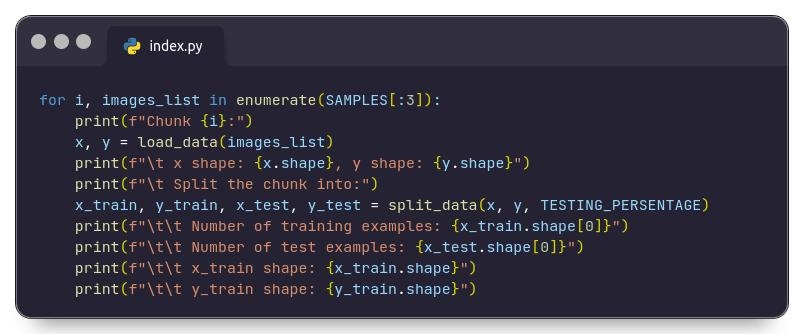
\includegraphics[width=0.90\textwidth]{Img/Chap-01/25.jpg}
    \caption{Training parameters}
    \label{fig:brain_tumor_train_params}
\end{figure}

\subsection{Loading and Splitting Data}

We load and split the data for training and testing. This is done for each chunk of data to handle large datasets efficiently, code snippet \ref{fig:brain_tumor_data_split}.

\begin{figure}
 \centering
    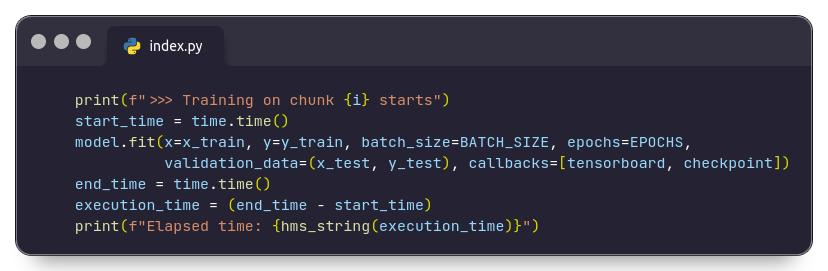
\includegraphics[width=0.90\textwidth]{Img/Chap-01/26.jpg}
    \caption{  Loading and Splitting the data}
    \label{fig:brain_tumor_data_split}
\end{figure}

\subsection{Training Loop}

We iterate over each chunk of data, train the model, and measure the time taken for training, code snippet \ref{fig:brain_tumor_training_loop}.

\begin{figure}
 \centering
    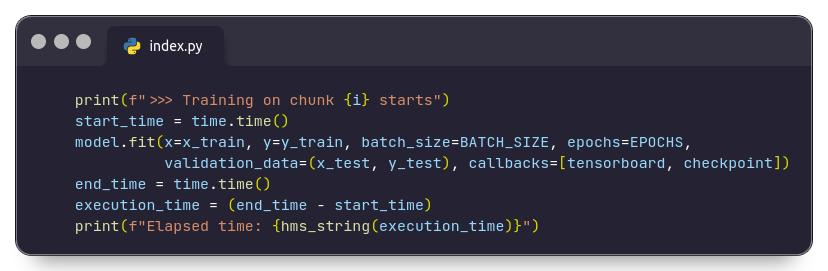
\includegraphics[width=0.90\textwidth]{Img/Chap-01/26.jpg}
    \caption{The Training Loop}
    \label{fig:brain_tumor_training_loop}
\end{figure}

\subsection{Summary}

In this section, we detailed the process of training the CNN model for brain tumor detection. We covered data loading, splitting, model training, and performance monitoring. 

By using callbacks, we ensured that the best model was saved, and the training process was logged for further analysis. The model's performance can be evaluated on the test set, and additional metrics such as the F1 score can be computed to assess its effectiveness.

\section{Brain Stroke detection model}
\subsection{Introduction}

In this section, we present the initial setup for our Brain Stroke Detection model, detailing the steps taken to prepare and process the dataset. T

his setup includes downloading the dataset, unzipping the files, and organizing the data into appropriate directories for normal and stroke CT scans. Additionally, we introduce sorting configurations to ensure the CT scan slices are correctly ordered for analysis. 

\subsection{Dataset Acquisition and Preparation}

To begin our model, we downloaded a dataset of brain CT scans from a public repository. This dataset is essential for training and evaluating our brain stroke detection model. The following code snippet illustrates the process of downloading and extracting the dataset, code snippet \ref{fig:brain_tumor_prep}.

\begin{figure}
 \centering
    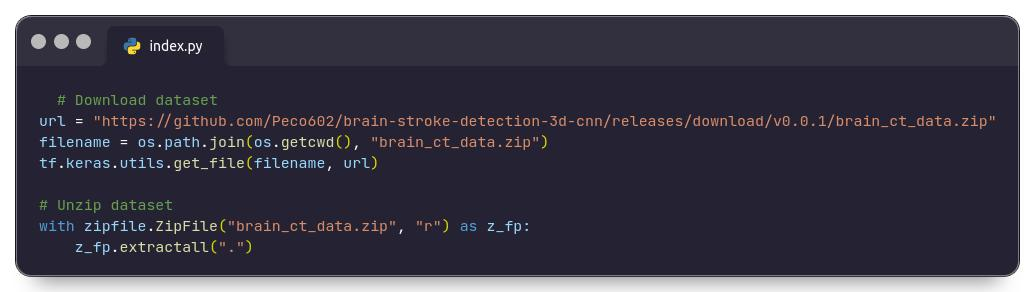
\includegraphics[width=0.90\textwidth]{Img/Chap-01/27.jpg}
    \caption{Dataset Acquisition and Preparation}
    \label{fig:brain_tumor_prep}
\end{figure}

This script utilizes TensorFlow's get file method to download the dataset from a specified URL. The dataset is then extracted into the current working directory using Python's `zipfile` module.

\subsection{Directory Structure}

Post extraction, the dataset is organized into separate directories for normal and stroke cases. The directory paths are defined as follows, code snippet \ref{fig:brain_tumor_datastructur}.
 
 \begin{figure}
 \centering
    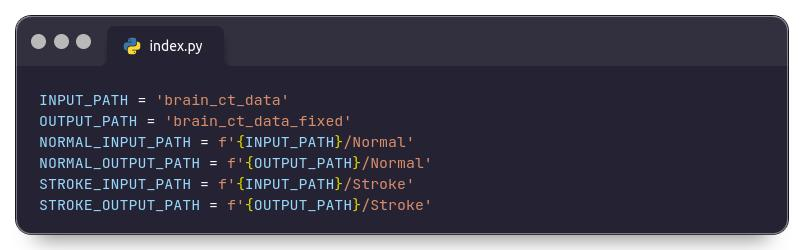
\includegraphics[width=0.90\textwidth]{Img/Chap-01/28.jpg}
    \caption{Data Directory Structure}
    \label{fig:brain_tumor_datastructur}
\end{figure}

\subsubsection{ Sorting Configuration }
 
Properly sorting the CT scan slices is crucial for accurate model training. The slices need to be ordered correctly to preserve the spatial information of the scans. We have implemented specific sorting configurations for both normal and stroke datasets. Below is an example of the sorting configuration for normal cases, code snippet \ref{fig:brain_stroke_norm_config}.
 

\begin{figure}
 \centering
    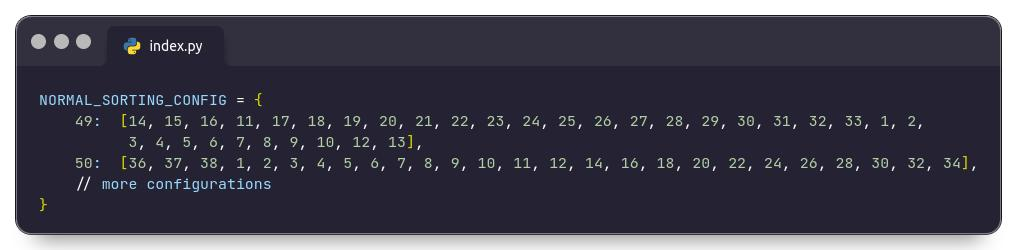
\includegraphics[width=0.90\textwidth]{Img/Chap-01/29.jpg}
    \caption{The normal sorting configuration}
    \label{fig:brain_stroke_norm_config}
\end{figure}

\subsection{Sorting Configuration}

The `NORMAL SORTING CONFIG` dictionary maps each patient identifier to a list of slice numbers in the correct order. Similarly, a sorting configuration is maintained for the stroke cases, code snippet \ref{fig:brain_stroke_sorting_config}.
 
\begin{figure}
 \centering
    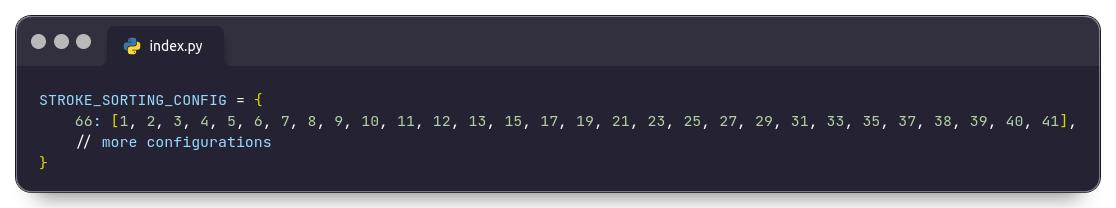
\includegraphics[width=0.90\textwidth]{Img/Chap-01/30.jpg}
    \caption{The stroke sorting configuration}
    \label{fig:brain_stroke_sorting_config}
\end{figure}

Each configuration ensures that the slices for a given patient are processed in the correct sequence, which is vital for maintaining the integrity of the 3D structure of the brain scans. 

\subsection{Dataset Preparation}

We have the count slices to analyze the slice's path and return a dictionary with the slice count associated with each patient, code snippet \ref{fig:brain_count_slice}.

\begin{figure}
 \centering
    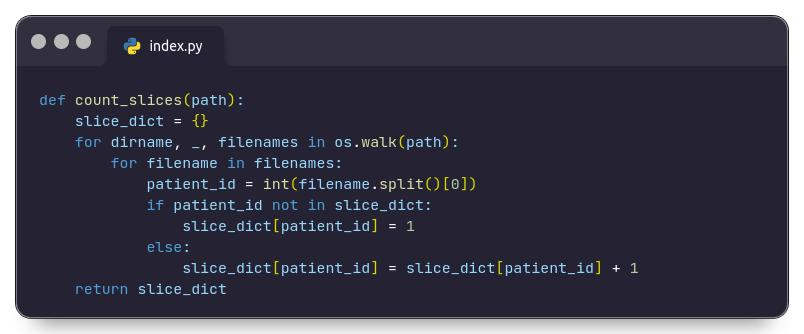
\includegraphics[width=0.90\textwidth]{Img/Chap-01/31.jpg}
    \caption{Count slices Function}
    \label{fig:brain_count_slice}
\end{figure}

and collect scan to load the scan per patient ID and prepare it, code snippet \ref{fig:brain_collect_slice}.

\begin{figure}
 \centering
    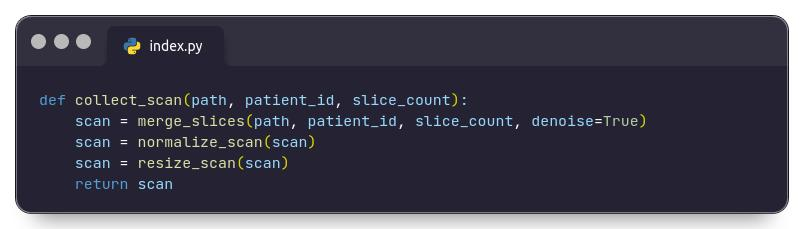
\includegraphics[width=0.90\textwidth]{Img/Chap-01/32.jpg}
    \caption{Collect Scans Function}
    \label{fig:brain_collect_slice}
\end{figure}

\subsection{Loading the Dataset}

We define a function to load the entire dataset into memory as a 4D array. Then we'll label it as stroke (1) or normal (0) and split the dataset into training and validation sets. 

\subsection{Data Augmentation}

We will use data augmentation techniques to increase the diversity of the training data without collecting new data. Augmentation helps improve the generalization capability of the model by artificially enlarging the dataset using random transformations.

The used techniques:
\begin{enumerate}
    \item \textbf{Rotation:} Slightly rotates images to simulate different angles of view.
    \item \textbf{Flipping:} Vertically flips images to increase variability.
    \item \textbf{Shifting:} Translates images along the x and y axes, creating different viewpoints.
    \item \textbf{Zooming:} Zooms in on images to simulate different focal lengths.
    \item \textbf{Shear Layer:} Distorts the image by slanting its shape, which can simulate perspective distortions.
    \item \textbf{Brightness Adjustment Layer:} Varies the brightness of the images, making them lighter or darker. 
    \item \textbf{Contrast Adjustment Layer:} Changes the contrast levels of the images, enhancing or reducing the difference between light and dark areas.
\end{enumerate}

\subsection{Building the model}

This chapter details the architecture of the 3D Convolutional Neural Network (CNN) model, including the augmentation layers and the process of compiling the model with appropriate loss functions, optimizers, and performance metrics.

\subsubsection{Model Parameters}

In our model, we have defined several key parameters that govern the architecture and training of our Convolutional Neural Network (CNN). These parameters are crucial for understanding how the model processes input data and how it learns from the data during training. Below is a detailed explanation of each parameter:

\begin{enumerate}
    \item Image Dimensions (WIDTH and HEIGHT):
        \begin{itemize}
            \item WIDTH = 128
            \item HEIGHT = 128
        \end{itemize}
         These parameters define the spatial dimensions of the input images fed into the CNN. Each image is resized or cropped to 128 pixels in width and 128 pixels in height. This standardization ensures that the input data is consistent in size, which is necessary for batch processing in the network. By using a fixed size, we also reduce computational complexity and memory usage.
    \item Input Depth (DEPTH) = 64
    This parameter specifies the number of channels in the input images. For typical RGB images, the depth would be 3 (corresponding to the red, green, and blue channels). However, in our project, the depth is set to 64, indicating that each input image consists of 64 feature channels. This could result from specific pre-processing steps or the use of specialized input data.
    \item Initial Learning Rate (INITIAL LEARNING RATE)  = 0.0001

    The learning rate is a critical hyperparameter that determines the step size during the optimization process. An initial learning rate of 0.0001 means that during the initial stages of training, the model's weights will be adjusted by this factor concerning the loss gradient. A small learning rate helps in making gradual updates, which can lead to more stable convergence.
    \item Learning Rate Decay Steps (DECAY STEPS) = 100000
    The decay steps parameter specifies the number of training steps after which the learning rate is decayed. In our model, after every 100000 steps, the learning rate is updated. This mechanism helps in gradually reducing the learning rate, allowing the model to fine-tune the weights as it approaches convergence.
    \item Learning Rate Decay Rate (DECAY RATE) = 0.96
    The decay rate defines the factor by which the learning rate is multiplied after each decay step. A decay rate of 0.96 means that the learning rate will be reduced by 4\% after every 100000 steps. This gradual reduction helps in maintaining a balance between convergence speed and the precision of the weight updates.
\end{enumerate}

\subsubsection{Model Building Function}

This section describes the architecture and implementation details of our CNN model designed for [your specific task, e.g., image classification, medical imaging, etc.]. The model leverages 3D convolutional layers to effectively capture spatial features from the input data.

\subparagraph{Model Parameters:}

\begin{itemize}
    \item Input Dimensions:
        \begin{itemize}
            \item Width: 128 pixels
            \item Height: 128 pixels
            \item Depth: 64 channels
        \end{itemize}
    \item Initial Learning Rate: 0.0001
    \item  Learning Rate Decay: Steps: 100000 -- Rate: 0.96
\end{itemize}

\subparagraph{Model Architecture:}

Our model consists of several layers designed to extract and process features from the input data:

\begin{enumerate}
    \item Input Layer: Accepts input images of shape (128, 128, 64).
    \item Reshape Layer: Adds an extra dimension to make the input suitable for 3D convolutions.
    \item Convolutional Layers: Four 3D convolutional layers with increasing filter sizes and ReLU activations.
    \item Pooling Layers: 3D max pooling layers to reduce spatial dimensions.
    \item Batch Normalization Layers: Normalize activations to improve training stability.
    \item Global Average Pooling: Reduces each feature map to a single value.
    \item Fully Connected Layer: Dense layer with 512 units and ReLU activation, followed by dropout for regularization.
    \item Output Layer: Single unit with sigmoid activation for binary classification.
\end{enumerate}

\subparagraph{Learning Rate Schedule:}

The learning rate decreases exponentially based on the specified decay steps and rate, allowing the model to fine-tune its weights as training progresses.

\subparagraph{Compilation:}

The model is compiled using the Adam optimizer with the defined learning rate schedule and binary cross-entropy loss. The performance is evaluated using specified metrics.

\subparagraph{Conclusion:}

This model is designed to effectively learn from high-dimensional input data and perform accurate binary classification. Further details on training procedures, data preprocessing, and evaluation metrics are discussed in subsequent sections.

\subsection{Model Training and Evaluation}

In this section, we cover the final step of the machine learning pipeline: training the model. This involves setting up callbacks for saving the best model, defining the training function, and training the model with different augmentation strategies. We aim to ensure the model learns effectively and generalizes well to unseen data.

\subsubsection{Setting the Number of Epochs}

The number of epochs determines how many times the model will iterate over the entire training dataset. Training for too few epochs might lead to underfitting, while too many epochs might cause overfitting. After careful consideration, we define the number of epochs as follows:

EPOCHS = 150

\subsubsection{Callback for Model Check pointing}

To ensure we save the best version of our model during training, we use a callback for model checkpointing. This callback monitors the validation AUC (Area Under the Curve) and saves the model weights whenever there is an improvement. This strategy helps in retaining the model that performs best on the validation set, preventing over-fitting and ensuring better generalization, code snippet \ref{fig:brain_model_checkpoint}.

\begin{figure}
 \centering
    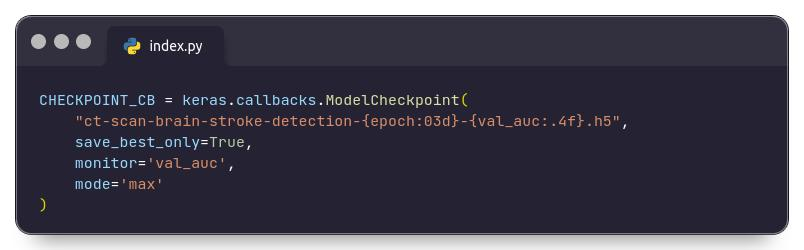
\includegraphics[width=0.90\textwidth]{Img/Chap-01/35.jpg}
    \caption{Setup the model checkpoint}
    \label{fig:brain_model_checkpoint}
\end{figure}

\subsubsection{Training Function}

We define a function \ref{fig:brain_strock_train} to encapsulate the training process. This function takes the model, training dataset, validation dataset, number of epochs, and any callbacks as input parameters. It then trains the model, performs validation at the end of each epoch, and returns the training history for further analysis.

\begin{figure}
 \centering
    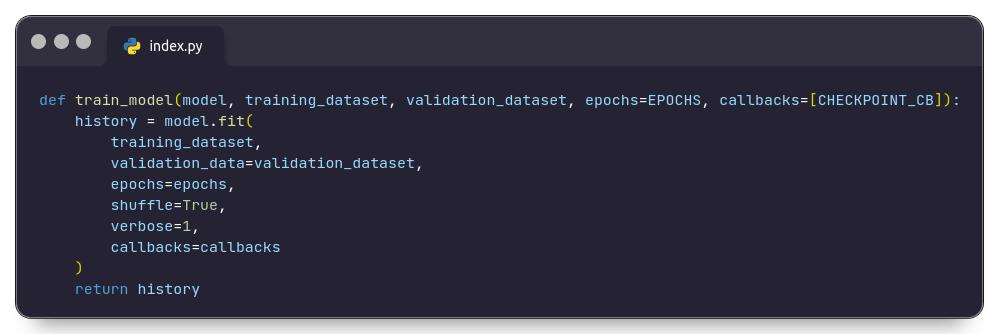
\includegraphics[width=0.90\textwidth]{Img/Chap-01/36.jpg}
    \caption{The training Function }
    \label{fig:brain_strock_train}
\end{figure}

\subsubsection{Conclusion}
This chapter outlines the comprehensive steps involved in training and evaluating our CNN model. By setting up proper callbacks, defining a robust training function, and applying data augmentation techniques, we aim to develop a model that not only performs well on the training data but also generalizes effectively to new, unseen data. The next chapter will delve into the results of our training process and discuss the model's performance on the test dataset.

%%%%%%%%%%%%%%%%%%%%%%%%%%%%%%%%%%%%%%%%%%%%%%%%%%%%%%%%%%%%%%%%%%%%%%%

\section{Overview of the Website}
\subsection{Tools, Technologies, and Techniques}
 
There are numerous tools and techniques available to aid in the completion of tasks and the execution of processes.

Integrated Development Environment (IDE) in which the source code can be implemented, such as Android Studio IDE, which will be used to develop the system using the Java programming language, as well as to design the Graphical User Interface (GUI) allowing interaction processes among system components.

Adobe Photoshop (UI) for designing the app's user interface, buttons, and layout.
Sketch (UX) to improve the user experience.

\subsubsection{GUI System}

\subparagraph{A GUI (Graphical User Interface)}
 is a system of interactive visual components for computer software. A GUI displays objects that convey information and represent actions that can be taken by the user. The objects change color, size, or visibility when the user interacts with them.

\subparagraph{GUI overview:}
A GUI includes GUI objects, like icons, cursors, and buttons. These graphical elements are sometimes enhanced with sounds, or visual effects like transparency and drop shadows. Using these objects, a user can use the computer without having to know commands.

\subparagraph{What are the elements of a GUI?}
To make a GUI as user-friendly as possible, there are different elements and objects that the user uses to interact with the software. Below is a list of each of these with a brief description.

\begin{itemize}
    \item \textbf{Button}: A graphical representation of a button that acts as a program when pressed.
    \item \textbf{Dialog box}: A type of window that displays additional information and asks a user for input.
    \item \textbf{Icon}: Small graphical representation of a program, feature, or file.
    \item \textbf{Menu}: List of commands or choices offered to the user through the menu bar.
    \item \textbf{Menu bar}: Thin, horizontal bar containing the labels of menus.
    \item \textbf{Ribbon}: Replacement for the file menu and toolbar that groups programs' activities together.
    \item \textbf{Tab}: Clickable area at the top of a window that shows another page or area.
    \item \textbf{Toolbar}: Row of buttons, often near the top of an application window that controls software functions.
    \item \textbf{Window}: Rectangular section of the computer's display that shows the program currently being used.
\end{itemize}

\subparagraph{How does a GUI work?}
A GUI uses windows, icons, and menus to carry out commands, such as opening, deleting, and moving files. Although a GUI operating system is primarily navigated using a mouse, a keyboard can also be used via keyboard shortcuts or arrow keys.

For example, if you want to open a program on a GUI system, you would move the mouse pointer to the program's icon and double-click it. With a command line interface, you need to know the commands to navigate to the directory containing the program, list the files, and then run the file.

\subparagraph{What are the benefits of GUI?}
A GUI is more user-friendly than a text-based command-line interface, such as MS-DOS, or the shell of Unix-like operating systems. 

Unlike a command-line operating system or CUI, like Unix or MS-DOS, GUI operating systems are easier to learn and use because commands do not need to be memorized. Additionally, users do not need to know any programming languages. Because of their ease of use and more modern appearance, GUI operating systems have come to dominate today's market.

 \subsubsection{Technologies}
 
\subparagraph{Front End:}
\begin{itemize}
    \item \textbf{HTML}
    
    HTML is essential for creating the structure of web pages. By using tags and attributes, you can create headings, paragraphs, links, images, and lists. It forms the foundation of web development, often used with CSS for styling and JavaScript for interactivity.
    
    \item \textbf{CSS}
    
    CSS is used to style HTML documents by defining rules that specify how elements should look. It enhances the visual presentation of web pages, allowing for the separation of content (HTML) from design (CSS). This separation makes it easier to maintain and update web pages.

    The framework used is Bootstrap, a versatile and powerful front-end framework that simplifies the process of designing responsive and modern web pages. Its grid system, pre-designed components, and utility classes allow developers to create attractive layouts quickly, while its JavaScript plugins add interactivity and enhance the user experience.
    
    \item \textbf{JavaScript}
    
    JavaScript is a versatile language essential for adding interactivity to web pages. It works alongside HTML and CSS to create dynamic user experiences, handle events, manipulate the DOM, and perform various client-side tasks. It allows developers to enhance the user experience by making web pages more engaging and responsive.

    Vue.js is a flexible and powerful framework for building interactive web interfaces. Its reactivity system, component-based architecture, and support for single-file components make it a popular choice for developers looking to create maintainable and efficient applications.
    
\end{itemize}

\paragraph{JAVASCRIPT code with explanation:}

\begin{figure}
 \centering
    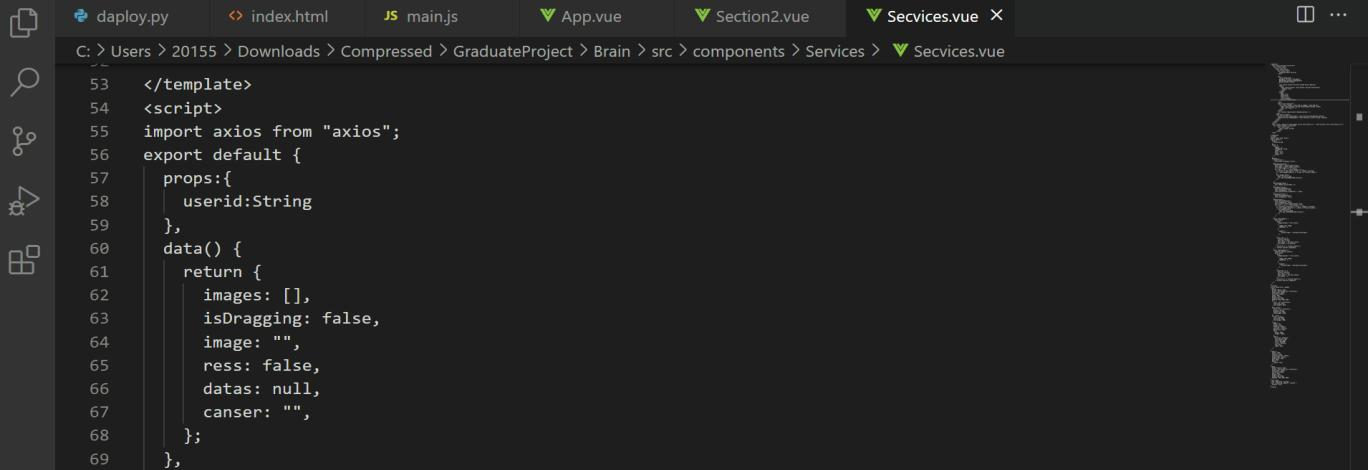
\includegraphics[width=0.90\textwidth]{Img/Chap-01/37.jpg}
    \caption{JS First code snippet}
    \label{fig:js_code_ex}
\end{figure}

As you see in \ref{fig:js_code_ex} and \ref{fig:js_code_ex2}, we did:

\begin{itemize}
    \item \textbf{import axios from "axios";}: This line imports the Axios library, which is a popular JavaScript library used to make HTTP requests.
    \item \textbf{export default { ... }}: This is the default export of the Vue component. Everything inside the curly braces defines the properties and behavior of the component.
    \item \textbf{props}: This is an object where we define the properties that the component accepts from its parent component.
    \item \textbf{userid}: String: This line defines a prop named user-id that is expected to be a string. This prop allows the parent component to pass a user-id value to this component.
    \item \textbf{data()}: This is a function that returns an object. This object contains the reactive data properties of the component.
    \item \textbf{images: []}: An empty array to hold images.
    \item \textbf{isDragging false}: A boolean flag that can be used to indicate if an item is being dragged (likely used in drag-and-drop functionality).
    \item \textbf{image: ""}: A string to hold the URL or data of a single image.
    \item \textbf{ress}: false: A boolean flag, its purpose isn't clear from this snippet alone but it's likely used to indicate some sort of state.
    \item \textbf{datas: null}: A variable to hold some data, initially set to null.
    \item \textbf{canser: ""}: A string variable, possibly meant to be canceled or something similar, but it's unclear without further context.
    \subparagraph{Purpose}: This method programmatically triggers a click event on a file input element.
Usage: It simulates a user clicking on a file input element to open the file picker dialog.
\end{itemize}

\begin{figure}
 \centering
    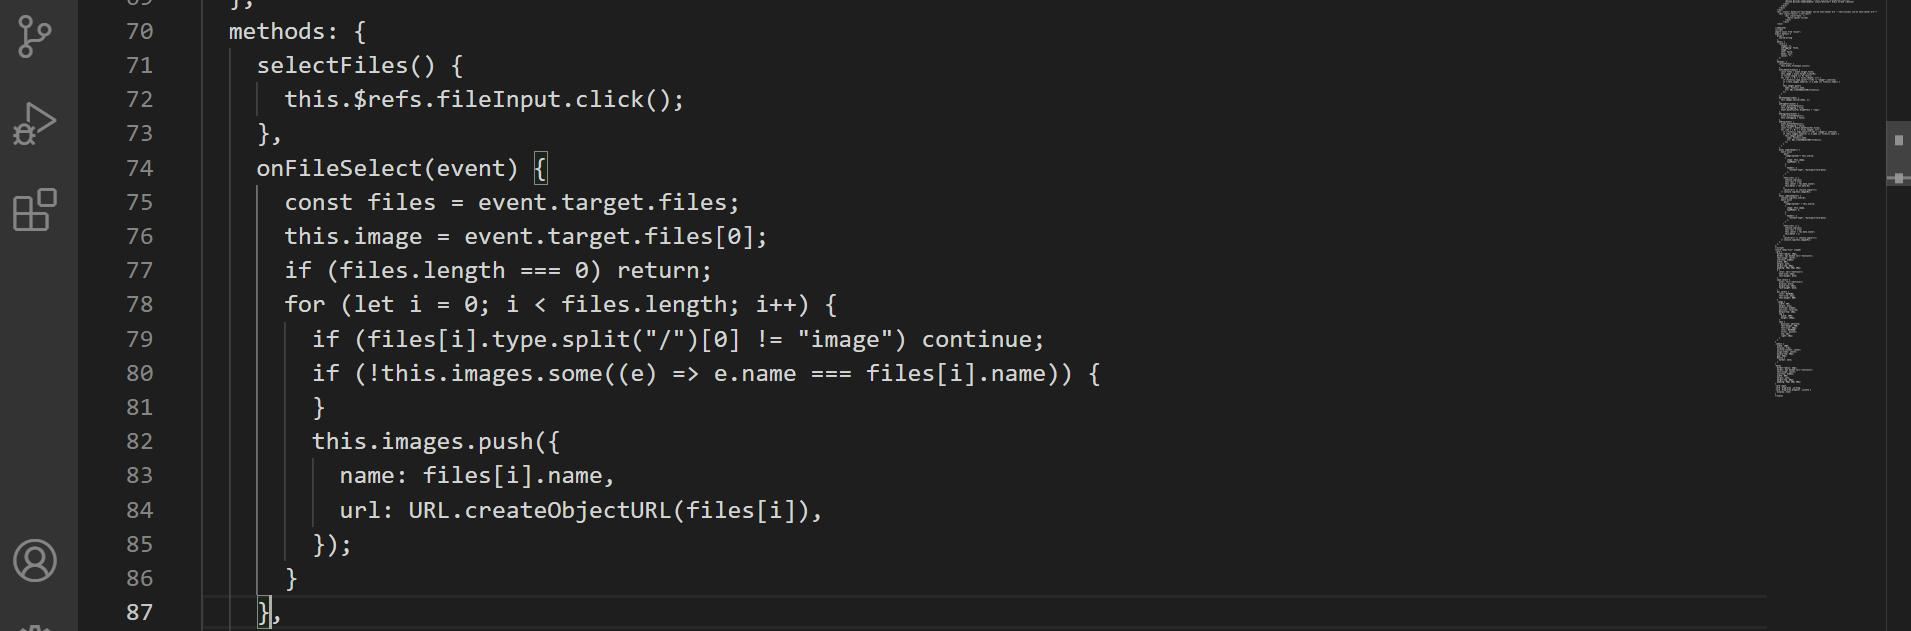
\includegraphics[width=0.90\textwidth]{Img/Chap-01/38.jpg}
    \caption{JS Secund code snippet}
    \label{fig:js_code_ex2}
\end{figure}

\paragraph{Back End:}
\begin{itemize}
    \item \textbf{Java}
    Java is a widely used, object-oriented programming language designed for building platform-independent applications. Its object-oriented nature, platform independence, and extensive libraries make it a popular choice for developers in various domains, from web and mobile development to enterprise systems.

    The framework used is Spring Boot, a powerful framework for building Spring-based applications with minimal setup and configuration. Its features like embedded servers, dependency management, and production-ready tools make it a popular choice for developing scalable and robust applications quickly.

    \item \textbf{Python}
    Python is a versatile and powerful language known for its simplicity and readability. It is widely used across various domains due to its extensive libraries, ease of use, and support for multiple programming paradigms.

    The framework used is Flask, a versatile and easy-to-use web framework for Python that allows for quick development of web applications, designed for building web applications quickly and with minimal setup. Its minimalist approach provides flexibility, while its support for extensions ensures that additional features can be easily integrated when needed.

    \item \textbf{Database (MySQL)}
    
    MySQL is a popular, open-source relational database management system known for its high performance and reliability. It is widely used in web development due to its ease of integration with various programming languages and its strong support for handling large datasets efficiently.
    
\end{itemize}

\paragraph{Code explanation:}

We used several Python libraries to load and run the trained models, shown in \ref{fig:be_1}, \ref{fig:ba_2}, \ref{fig:be_3}, \ref{fig:be_4}, \ref{fig:be_5}, \ref{fig:be_6} and \ref{fig:be_7}.

\begin{figure}
 \centering
    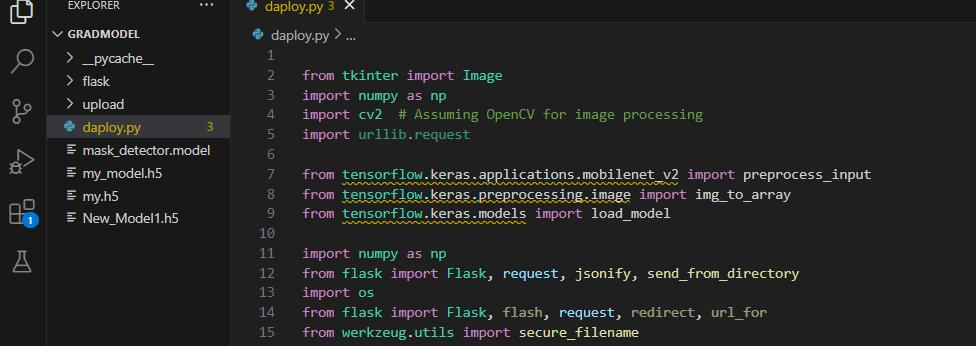
\includegraphics[width=0.90\textwidth]{Img/Chap-01/42.jpg}
    \caption{Used Python libraries}
    \label{fig:be_1}
\end{figure}

\paragraph{Which contains:}
\subparagraph{tkinter (Image):}
 Although Image is not typically imported directly from tkinter, this library is generally used for creating graphical user interfaces (GUIs). You might be referring to `PIL.Image` from the Pillow library for image processing.
 
\subparagraph{NumPy (np):}
 A fundamental library for scientific computing in Python is used here for handling arrays and matrices.
 
\subparagraph{cv2 (OpenCV):}
 An open-source computer vision library. It provides tools for image processing and computer vision tasks.
\subparagraph{urllib.request:}
 A module for opening and reading URLs. Often used to fetch data from the web.
\subparagraph{`tensorflow.keras.applications.mobilenet` v2 (preprocess input):}
 Part of TensorFlow’s Keras module, this provides functions to preprocess input data for the MobileNetV2 model.

\subparagraph{`tensorflow.keras.preprocessing.image` (img to array):}
 Utility for converting a PIL Image instance to a Numpy array.
\subparagraph{tensorflow.keras.models (load model):}
 Provides functions to load pre-trained Keras models.
\subparagraph{Flask:}
 A lightweight WSGI web application framework in Python, used for creating web applications and APIs.
os: A module providing a way of using operating system-dependent functionality like reading or writing to the file system.

\subparagraph{werkzeug.utils (secure filename):}
 A utility for securing a filename before storing it directly on the filesystem.


\begin{figure}
    \centering
    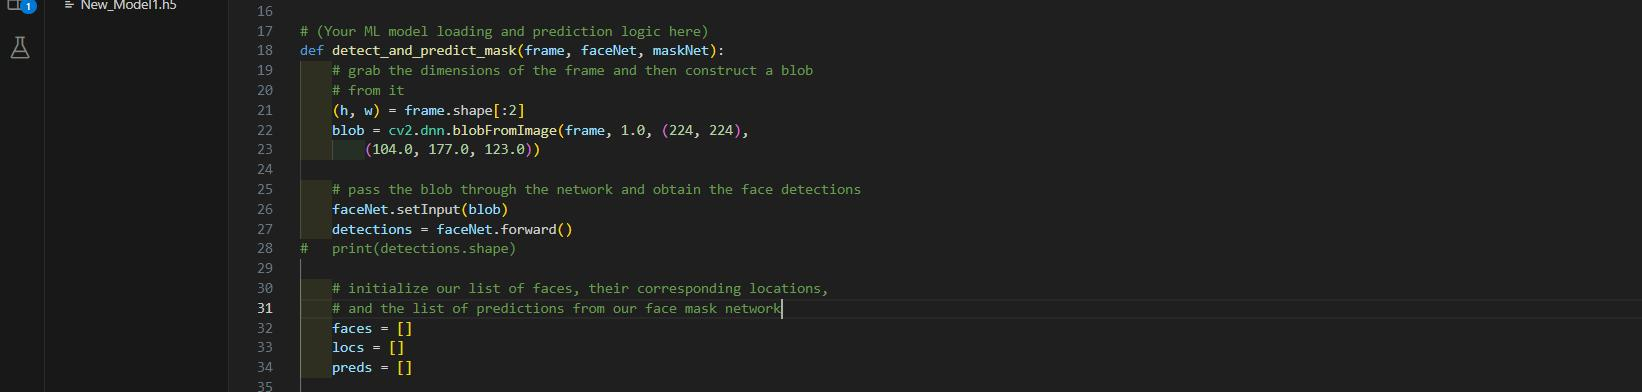
\includegraphics[width=0.90\textwidth]{Img/Chap-01/43.jpg}
    \caption{Detect and Predict Mask Function}
    \label{fig:ba_2}
\end{figure}

\begin{itemize}
    \item \textbf{frame}: The input image frame where face masks need to be detected.
    \item \textbf{faceNet}: The pre-trained deep learning model used for face detection.
    \item \textbf{maskNet}: The pre-trained deep learning model used for face mask classification.
    \item It extracts the height and width of the input frame.
    \item \textbf{blobFromImage function} of OpenCV's CNN module is used to preprocess the frame:
    \begin{itemize}
        \item It resizes the image to (224, 224) pixels.
        \item Normalizes the pixel intensities.
        \item Converts the image to a blob format suitable for input to a neural network.
    \end{itemize}
    \item The pre-trained faceNet model is used to detect faces in the image.
    \item The preprocessed blob is set as the input to the faceNet model.
    \item The forward method is called to perform forward pass inference, obtaining face detections.
\end{itemize}

\begin{figure}
    \centering
    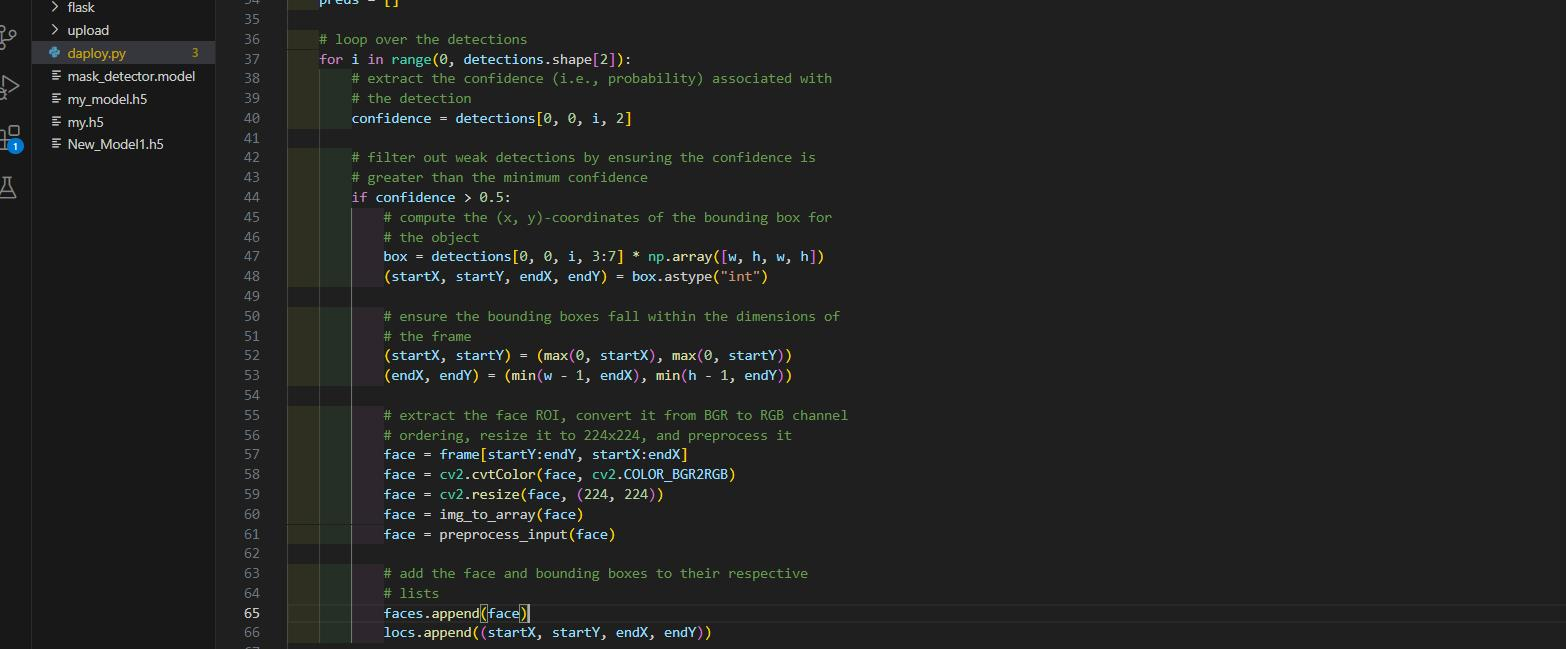
\includegraphics[width=0.90\textwidth]{Img/Chap-01/44.jpg}
    \caption{Loop over detictions}
    \label{fig:be_3}
\end{figure}

\begin{itemize}
    \item Iterates over the detections found by the face detection model.
    \item Extracts the confidence (probability) associated with the detection.
    \item Filters out weak detections by ensuring the confidence is greater than a minimum threshold (here, 0.5).
    \item Computes the (x, y)-coordinates of the bounding box for the detected face. The bounding box coordinates are relative to the dimensions of the input frame.
    \item Ensures that the bounding boxes fall within the dimensions of the frame to prevent errors.
    \item Extracts the face region from the frame.
    \item Converts the color space of the face region from BGR to RGB.
    \item Resizes the face region to the required input size (224x224) for the mask classification model.
    \item Converts the face region to a NumPy array and preprocesses it for the model.
    \item Adds the preprocessed face and its bounding box coordinates to their respective lists for further processing.
\end{itemize}

\begin{figure}
    \centering
    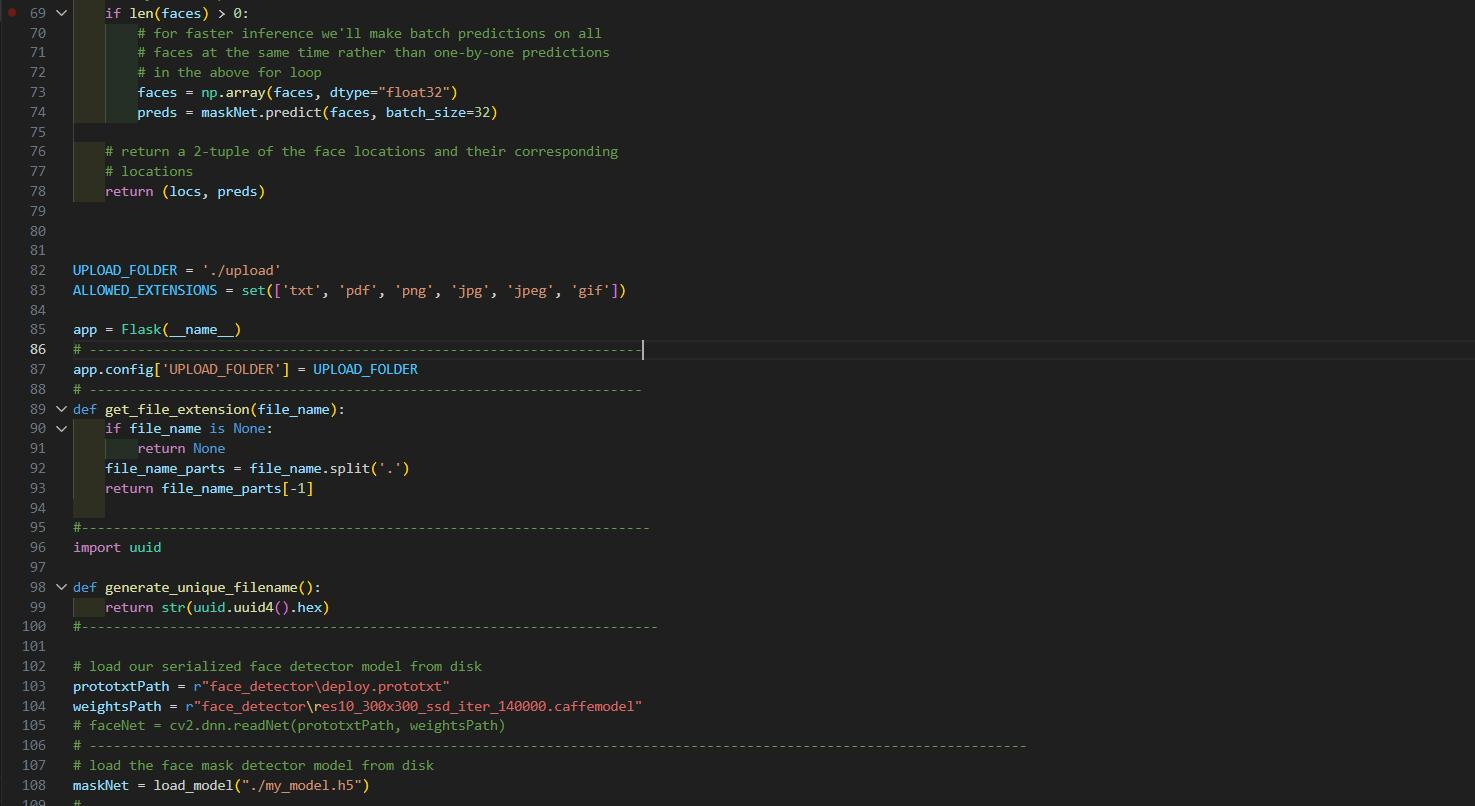
\includegraphics[width=0.90\textwidth]{Img/Chap-01/45.jpg}
    \caption{Load the trained model}
    \label{fig:be_4}
\end{figure}

\begin{itemize}
    \item If there are detected faces, it converts the list of faces into a NumPy array.
    \item It then uses the prediction method of the mask detection model (maskNet) to predict whether each face is wearing a mask or not. This is done in batch mode for faster processing.
    \item Returns a tuple containing the locations of the detected faces and their corresponding predictions regarding whether they are wearing masks or not.
    \item Set up configurations for handling uploaded files, including the allowed file extensions and the upload folder.
    \item Defines a utility function to extract the file extension from a given file name.
    \item Defines a utility function to generate a unique filename using the UUID module.
    \item Loads the face detection model (prototxtPath and weightsPath) and the face mask detection model (maskNet) from disk.
    \item The face detection model seems to be based on the Caffe framework, and the face mask detection model is loaded using Keras's load model function.
\end{itemize}

\begin{figure}
    \centering
    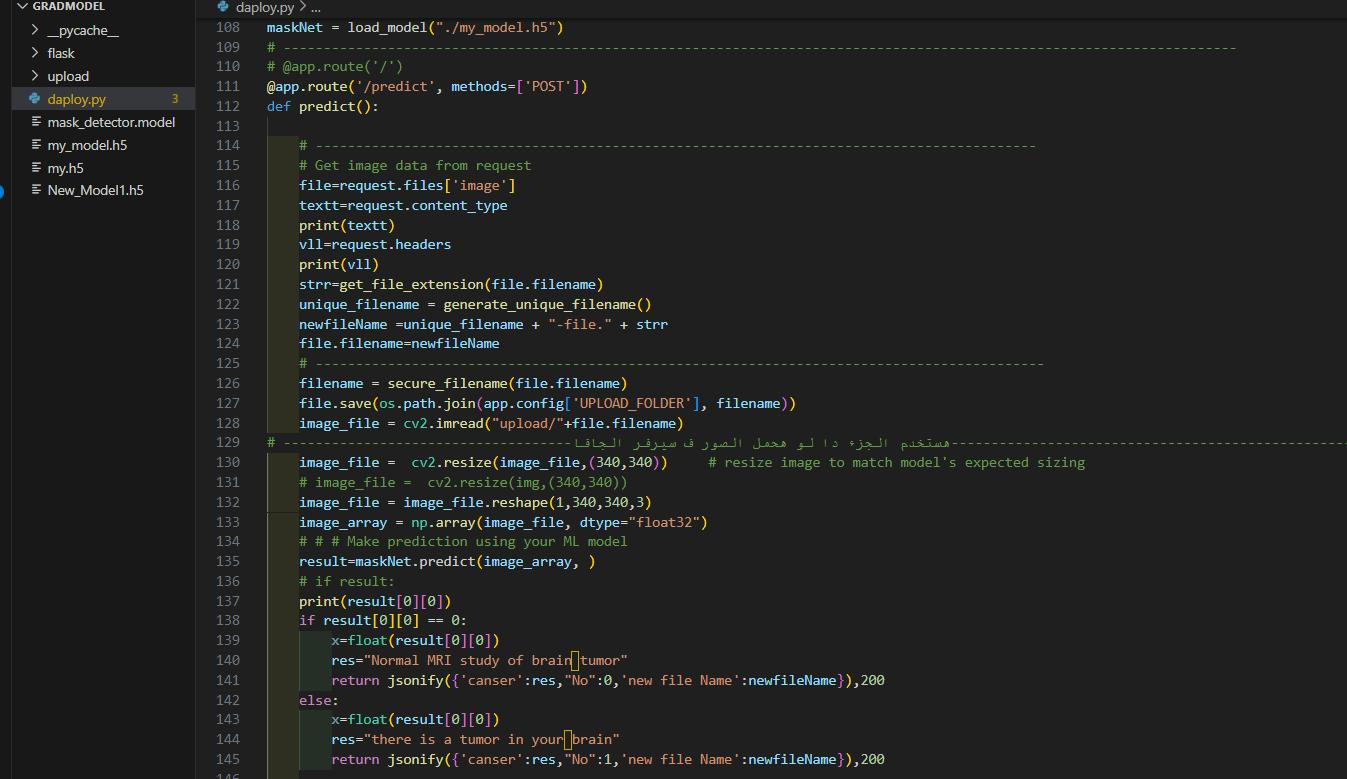
\includegraphics[width=0.90\textwidth]{Img/Chap-01/46.jpg}
    \caption{The main API entry point}
    \label{fig:be_5}
\end{figure}

\begin{itemize}
    \item Retrieves the image file from the request.
    \item Collects information about the content type and headers of the request.
    \item Generates a unique filename for the uploaded image.
    \item Saves the uploaded image with the generated filename in the upload folder specified in the application's configuration.
    \item Reads the uploaded image using OpenCV (cv2).
    \item Resizes the image to match the expected input size of the model.
    \item Prepares the image array for prediction.
    \item Uses the trained machine learning model (maskNet) to predict the class of the input image.
    \item Based on the prediction result, it returns a JSON response indicating whether the image depicts a normal MRI study or if there's a tumor in the brain. It also includes the new filename generated for the uploaded image.
\end{itemize}

\begin{figure}
    \centering
    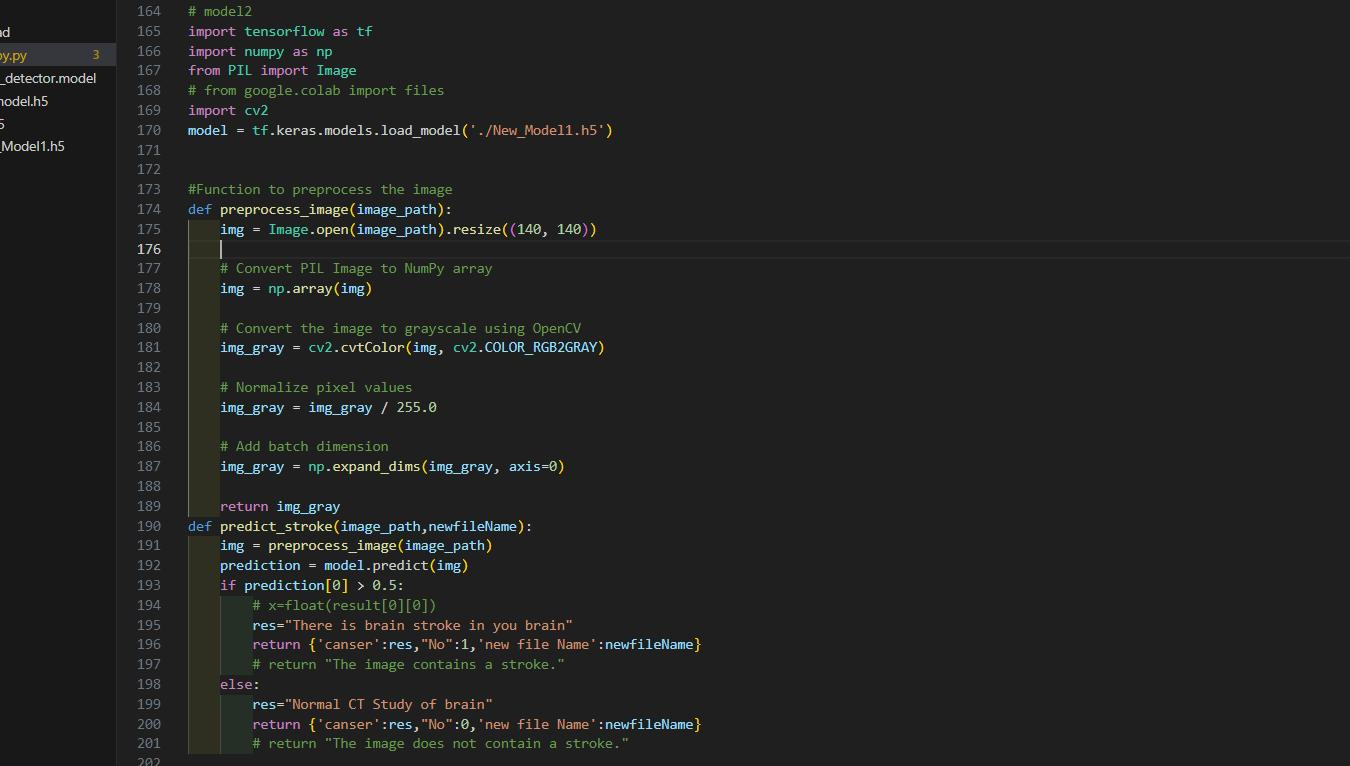
\includegraphics[width=0.90\textwidth]{Img/Chap-01/47.jpg}
    \caption{Pre-process the user input}
    \label{fig:be_6}
\end{figure}

\begin{itemize}
    \item TensorFlow (tf) for loading the machine learning model.
    \item NumPy (np) for numerical operations.
    \item PIL (Image) for image manipulation.
    \item OpenCV (cv2) for image processing.
    \item Loads a trained Keras model from the specified file (New Model1.h5).
    \item Resizes the image to (140, 140) pixels.
    \item Converts the image to grayscale using OpenCV.
    \item Normalizes pixel values to the range [0, 1].
    \item Adds a batch dimension to the image.
    \item Preprocesses the input image using the preprocess image function.
    \item Uses the loaded model to predict whether the image contains a stroke.
    \item Returns a dictionary indicating the prediction result along with the new filename.
    \item Checks if the model prediction is greater than 0.5.
    \item If the prediction is greater, it suggests that the image contains a stroke; otherwise, it suggests the image is normal.
    \item Returns a dictionary containing the prediction result (res), a flag (No) indicating the presence of stroke (1) or absence (0), and the new filename for the uploaded image.
\end{itemize}

\begin{figure}
    \centering
    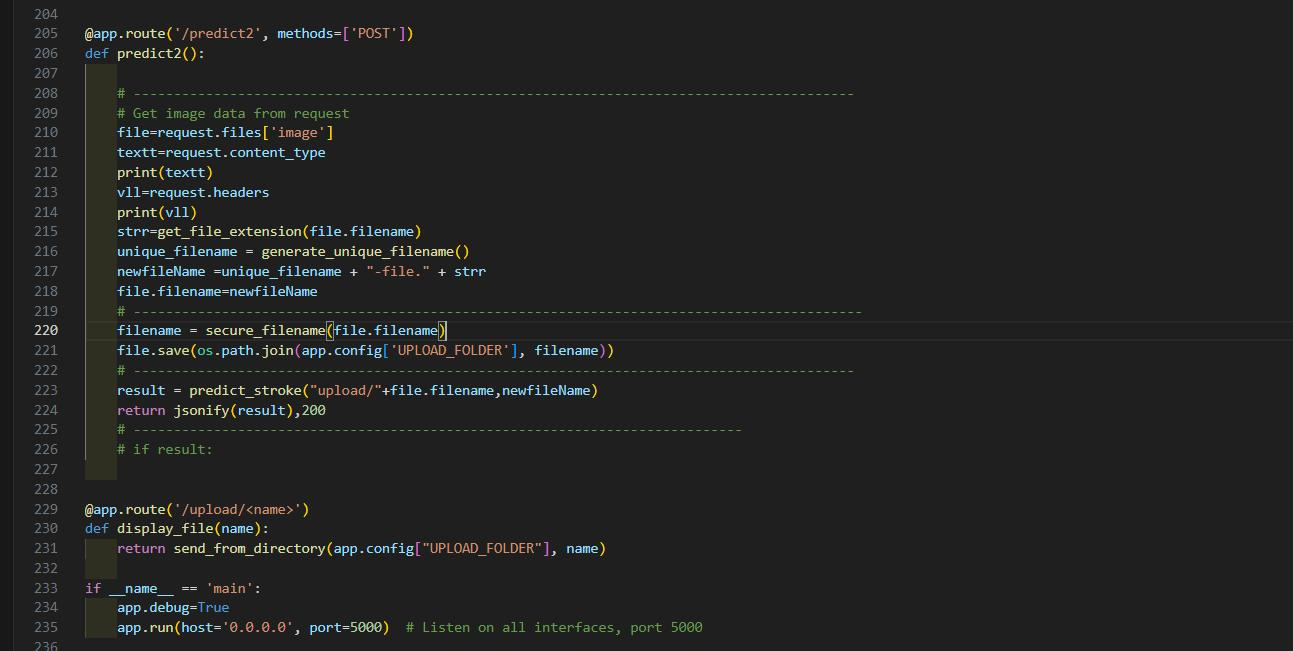
\includegraphics[width=0.90\textwidth]{Img/Chap-01/48.jpg}
    \caption{The prediction API entry point}
    \label{fig:be_7}
\end{figure}

\begin{itemize}
    \item Defines a new route /predict2 that listens for POST requests.
    \item Retrieves the image file from the request.
    \item Collects information about the content type and headers of the request.
    \item Generates a unique filename for the uploaded image.
    \item Saves the uploaded image with the generated filename in the upload folder specified in the application's configuration.
    \item Calls the predict stroke function to predict whether the image contains a brain stroke.
    \item Returns the prediction result as a JSON response along with an HTTP status code indicating success.
    \item Defines a route /upload/<name> to display uploaded files.
    \item The function display file retrieves the file with the given filename from the upload folder and sends it to the client.
    \item Runs the Flask application on the specified host and port (0.0.0.0:5000).
\end{itemize}


